\documentclass[12pt]{exam}

\usepackage{graphicx}
\usepackage{url}
\usepackage{comment}

\usepackage{geometry}
\usepackage{multicol}
\usepackage{relsize}

\geometry{
  %includeheadfoot,
  margin=2.54cm
}

\usepackage{fancyvrb}

\fvset{tabsize=2}
%\fvset{fontsize=\relsize{-1}}
\fvset{frame=single}

\begin{document}
\section*{Programming Paradigms --- Erlang Lab sheet}

Here are some simple exercises to get you started with Erlang. 
As you have already worked with a functional language the exercises about lists should be particularly familiar.
\begin{questions}
\question\label{first}
Suppose that the weekly income of ``Burger Bar'' is given by some function \texttt{sales} which takes a 
week number as an argument and returns the income for that week. 
Consider the following function:
\begin{Verbatim}
sales(N) ->  (N + 31) rem 7  +  (N + 1) rem 5.
\end{Verbatim}
\begin{parts}
\part
Define a function which given a week number \texttt{n} returns the number of weeks in the range \texttt{0,...,n} 
for which the sales were 0.
\part
Define a function which given a week number \texttt{n} and a number \texttt{s} returns the number of 
weeks in the range \texttt{0,...,n} for which the sales where higher than \texttt{s}.
\part
Define the function \texttt{allZeroPeriod(N)} such that \texttt{allZeroPeriod} tests whether the sales for 
every week in the range $0 to n$ are zero.
\part
Define a function which given a week number \texttt{n} finds the week in the range \texttt{0,...,n} 
which had the maximum sales. Don't forget that you can define \emph{helper} functions.
\end{parts}

\question
The \texttt{factorial} function from the quick-start guide has a simple recursive form 
but it is not the most efficient structure. 
To write recursive functions efficiently in Erlang they must be \emph{tail recursive}. 

[Remember: A function is tail recursive (roughly speaking) if for any recursive call the answer 
returned by the recursive call is the whole answer.]

The following version of \texttt{factorial} is not tail recursive:
\begin{Verbatim}
-module(test).
-export([fac/1]).

fac(0) -> 1;
fac(N) -> N * fac(N-1).
\end{Verbatim}
It is not tail recursive because the recursive call \texttt{fac(N-1)} is not the whole result 
– it has to be multiplied by \texttt{N}.

Here is the equivalent tail recursive version. 
\begin{Verbatim}
-module(test).
-export([fac/1]).
fac(N) -> fac(N,1).

fac(0,A) -> A;
fac(N,A) -> fac(N-1,N*A).
\end{Verbatim}
This is tail recursive, since the result of the recursive call \texttt{fac(N-1,N*A)} is the whole result.

Now rewrite one of your non tail recursive solutions to Question~\ref{first} to be tail recursive.

\question
\begin{parts}
\part
Write a function \texttt{increasing} which takes any list of pairs of numbers, and returns a list of 
only those pairs from the original list for which the first element is smaller than the second element.
\part
Write a function \texttt{changePairs} which takes any list of pairs of numbers, and returns the 
list in which all of the second elements have been replaced by the largest second element. For example,

\verb!changePairs [{1,2},{7,5},{6,3}]! gives \verb![{1,5},{7,5},{6,5}]!
\end{parts}

\question
\begin{parts}
\part
Write a program which creates a process and sends a message to that process. 
The created process should print out the message.
\part
Modify the above program so that you can send any number of messages to the process, 
each of which will be printed out.
\part
Further modify the program so that it swaps adjacent messages, so if you send it the sequence 
\texttt{1, 2, 3, 4} it will print out \texttt{2, 1, 4, 3}.
\end{parts}

\question
Implement the prime number sieve using the a pipeline algorithm.
\begin{itemize}
\item
The main process creates the first filter process and sends it a sequence of natural numbers starting with 2.
\item
A printer process writes the prime numbers that it receives to the output.
\item
Each process in the filter pipeline has the following behaviour: 
\begin{itemize}
\item
It sends the first number that it receives to the printer process, and keeps a copy of that number \texttt{P}. 
\item
It creates the next process in the pipeline, and then forwards every number 
it receives which is not divisible by the first number \texttt{P} (use the \texttt{rem} operator).
\end{itemize}
It is a good idea to decide in advance how far you want to search, and to terminate the filters when you are finished.
\end{itemize}

\question
Write a function \texttt{sign(N)} (in a module \texttt{mymodule})
that gets a number \texttt{N} as an input parameter and outputs
-1 if \texttt{N} is negative, 1 if \texttt{N} is positive, and
0 if \texttt{N} is equal to zero.

\begin{solutionorbox}
\begin{verbatim}
-module(mymodule).
-export([sign/1]).

sign(N) -> 
  if 
    N > 0 -> 1;
    N < 0 -> -1;
    N == 0 -> 0
  end.
\end{verbatim}

Alternatively, you can add a guard to make sure that the
comparisons in the \texttt{if} statement are only done if
\texttt{N} is a number:

\begin{verbatim}
-module(mymodule2).
-export([sign/1]).

sign(N) when is_number(N) -> 
  if 
    N > 0 -> 1;
    N < 0 -> -1;
    N == 0 -> 0
  end;
sign(N) ->
  "not a number".
\end{verbatim}
\end{solutionorbox}

\question

\begin{parts}

\part\label{one}
In a module \texttt{greeter} write a function \texttt{hello} with
one input parameter \texttt{Name}. The output of the function
should be ``Hello $<$Name$>$!'' on the console. (Remember:
the Erlang command for printing is

\begin{Verbatim}
io:format("...~p...~p...", [param1,...,paramn]).
\end{Verbatim}

where every placeholder \texttt{p} in the format string
will be replaced by the corresponding list item
\texttt{param}.

\begin{solutionorbox}
\begin{verbatim}
-module(greeter).
-export([hello/1]).

hello(Name) ->
  io:format("Hello ~p!~n",[Name]).
\end{verbatim}
\end{solutionorbox}

\part\label{two}
In the console write an anonymous function that does
the same as in (\ref{one}) and assign it to a variable. Now
call the function using the variable.

\begin{solutionorbox}
\begin{verbatim}
Greeter = fun(Name) -> io:format("Hello ~p!~n",[Name]) end.
Greeter(John).
\end{verbatim}
\end{solutionorbox}

\part
Use the anonymous function in (\ref{two}) and apply it to a list,
greeting every element in the list.

\begin{solutionorbox}
\begin{verbatim}
lists:foreach(fun(Name) -> 
  io:format("Hello ~p!~n",[Name]) end, [1,2,3,4,5]).
\end{verbatim}
\end{solutionorbox}

\end{parts}

\question

\begin{parts}

\part
Write a function \texttt{listaux:min} that returns the 
minimum element of the list. Given the list
\texttt{[3,2,9,4,5]}, \texttt{listaux:min} would output
\texttt{2}. 

Hint: first write
a function \texttt{listaux:checkmin(X,Y)} that returns
the minimum of two values \texttt{X} and \texttt{Y}. This
function can then be used as the function parameter 
for a \texttt{fold} function. 

The syntax for passing
a non-anonymous function to a \texttt{fold} function is
the following:

\begin{Verbatim}
lists:foldl(fun listaux:checkmin/2,...,...)
\end{Verbatim}

If you cannot manage to write the \texttt{checkmin}
function, you can use the built-in function
\texttt{erlang:min}.)

\part 
Write a function \texttt{listaux:max} that returns the 
maximum element of the list. Given the list
\texttt{[3,2,9,4,5]}, \texttt{listaux:max} would output
\texttt{9}.

\part
Write a function \texttt{listaux:minmax} that returns a
tuple containing the minimum and the maximum element of
the list. Given the list
\texttt{[3,2,9,4,5]}, \texttt{listaux:minmax} would output
\texttt{\{2,9\}}.

\end{parts}

\begin{solutionorbox}
\begin{verbatim}
-module(listaux).
-export([min/1]).
-export([max/1]).
-export([minmax/1]).
-export([checkmin/2]).
-export([checkmax/2]).
-export([checkminmax/2]).

checkmin(Item,TmpMin) ->
  if 
    Item < TmpMin -> Item;
    true -> TmpMin
  end.

min([]) ->
  "no minimum, empty list";
min([H|T]) ->
  lists:foldl(fun listaux:checkmin/2,H,T).


checkmax(Item,TmpMin) ->
  if 
    Item > TmpMin -> Item;
    true -> TmpMin
  end.

max([]) ->
  "no minimum, empty list";
max([H|T]) ->
  lists:foldl(fun listaux:checkmax/2,H,T).


checkminmax(Item,{TmpMin,TmpMax}) ->
  if 
    Item < TmpMin -> {Item,TmpMax};
    Item > TmpMax -> {TmpMin,Item};
    true -> {TmpMin,TmpMax}
  end.

minmax([]) ->
  "no minmax, empty list";
minmax([H|T]) ->
  lists:foldl(fun listaux:checkminmax/2,{H,H},T).

\end{verbatim}
\end{solutionorbox}

\question
\begin{parts}
\part
  Write a function that just echoes whatever message it 
  receives via \texttt{io:format}, i.e., it will print any
  received message in the console. Start a process running
  this function and send it several messages from the
  interactive Erlang shell.
  
\begin{solutionorbox}
\begin{verbatim}
-module(echo).
-export([loop/0]).

loop() -> 
  receive
    X -> io:format("~p~n", [X]),
    loop()
  end.
\end{verbatim}

After compilation, start process with

\begin{verbatim}
EPid = spawn(fun echo:loop/0).
\end{verbatim}

and send messages via

\begin{verbatim}
EPid ! "hello".
\end{verbatim}
\end{solutionorbox}

\part\label{lab}
  Now change the function so that it does not output
  the received message, but sends it back to the sender.
  On the sending side write a function that sends a message,
  waits for the reply, and outputs the returned message
  (this function is similar to the \texttt{translate} function we looked at in class).

\begin{solutionorbox}
\begin{verbatim}
-module(echo2).
-export([loop/0]).
-export([send/2]).

loop() -> 
  receive
    {Pid,X} -> Pid,
    Pid ! X,
    loop()
  end.

send(To,Message) ->
  To ! {self(),Message},
  receive
    Y -> io:format("Message received: ~p~n", [Y])
  end.
\end{verbatim}


After compilation, start process with

\begin{verbatim}
EPid = spawn(fun echo2:loop/0).
\end{verbatim}

and send messages via

\begin{verbatim}
echo2:send(EPid2,"hello").
\end{verbatim}
\end{solutionorbox}

\part\label{nextLab}
  Change the function so that it does not return
  the received message, but computes the factorial of
  the message and sends this back. Send a couple of 
  numbers to the process via the send function you have
  written in part (\ref{lab}).

\begin{solutionorbox}
\begin{verbatim}
-module(server).
-export([server/0]).
-export([send/2]).


server() -> 
  receive
    {Pid,X} -> Pid ! fac(X),
    server()
  end.


send(To,Message) ->
  To ! {self(),Message},
  receive
    Y -> io:format("Message received: ~p~n", [Y])
  end.


fac(0) -> 1;
fac(N) -> N * fac(N-1).
\end{verbatim}

Start and send messages like in last example. Make sure that
you only send integers as messages.
\end{solutionorbox}

\part\label{lastLab}
  Write a function \texttt{client} that sends two messages
  containing the numbers 5 and 7 to the server implemented 
  in part (\ref{nextLab}) and prints out the result sent back from the
  server. After that the client process should just stop,
  i.e., not execute any other commands.   
  
  (Hint: first start
  the server process and bind it to an atom, e.g. \texttt{facserver},
  which is used by the client function as recipient of 
  the messages. Then start the client process to see what
  happens.)

\part 
 Expand the functions from part (\ref{lastLab}) by going through a
 simplified three-way handshake before sending the
 requests from the client side. (Simplified handshake
 means that you only need to implement the messages that
 get passed back and forth in a successful handshake, 
 and not implement the actual functionality.) 
 
 After sending the two
 requests (numbers 5 and 7) terminate the connection
 by sending \texttt{finalize} messages. See Figure \ref{fig:threeway}
 for a diagram.



\begin{solutionorbox}
\begin{verbatim}
-module(clisrv).
-export([server/0]).
-export([client/0]).


server() -> 
  receive
    {Pid,X} -> Pid ! fac(X),
    server()
  end.


client() ->
  facsrv ! {self(),5},
  receive
    Y1 -> io:format("Message received: ~p~n", [Y1])
  end,
  facsrv ! {self(),10},
  receive
    Y2 -> io:format("Message received: ~p~n", [Y2])
  end.
  

fac(0) -> 1;
fac(N) -> N * fac(N-1).
\end{verbatim}


Start server with

\begin{verbatim}
register(facsrv,spawn(fun clisrv:server/0)).
\end{verbatim}

and start client with

\begin{verbatim}
spawn(fun clisrv:client/0).
\end{verbatim}
\end{solutionorbox}

\end{parts}

\end{questions}

\begin{figure}[htb]
\begin{center}
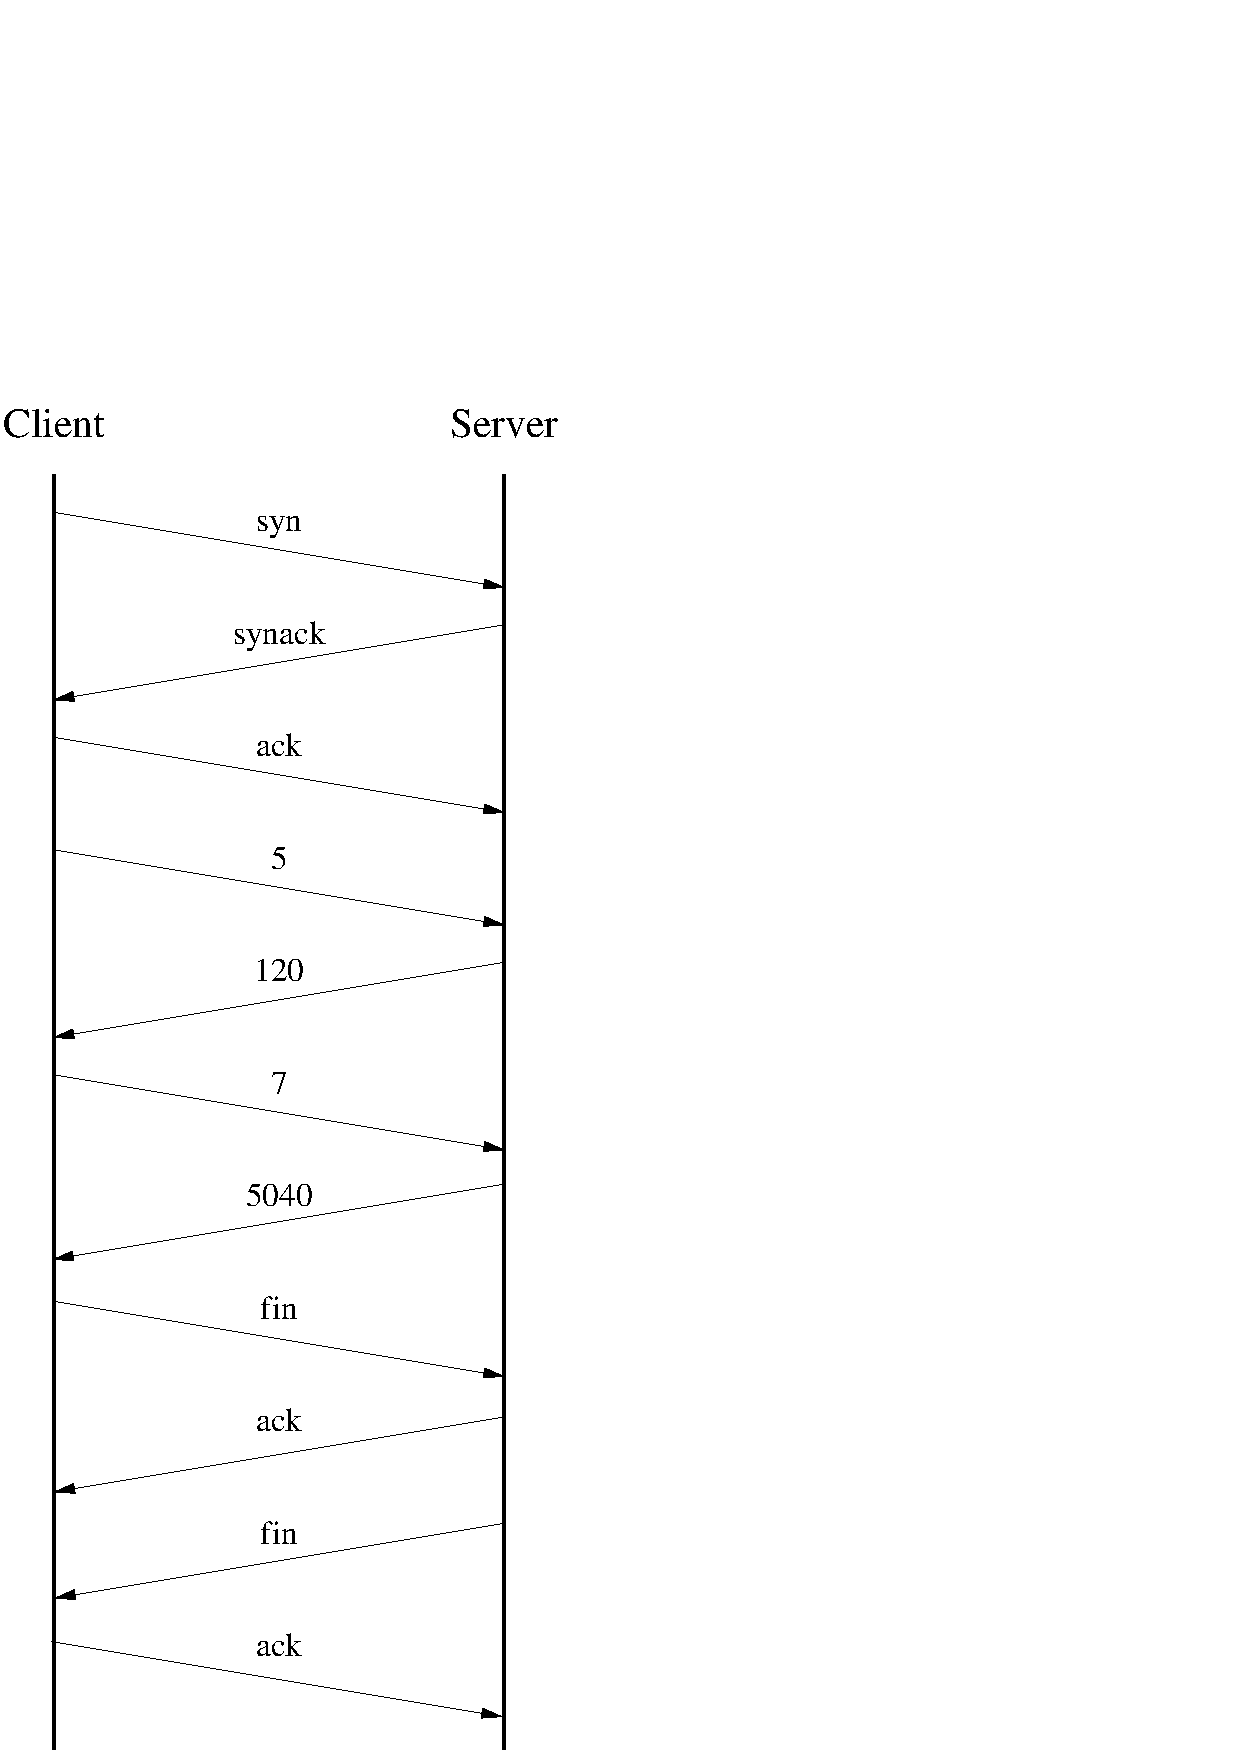
\includegraphics[scale=0.5]{images/ex7diagram.png}
\end{center}
\caption{Handshake between client and server}
\label{fig:threeway}
\end{figure}


\section*{Credits}
Thanks to Kvs Prasad at G\"{o}teborg University and Sven Helmer for collaborating on these questions.
Some of these questions were \emph{inspired} by materials at \url{erlang.org}.
\end{document}